\documentclass[12pt,fleqn]{article}\usepackage{../../common}
\begin{document}
Toplu Tavsiye (Collaborative Filtering), Filmler, SVD ile Boyut İndirgeme

Film tavsiye verilerine kullanarak bazı analizler ve tavsiye yaklaşımlarına
bakacağız. Diyelim ki Star Trek (ST) dizisini ne kadar beğendiğini 4 tane
kullanıcı sezonlara göre işaretlemiş. Bu örnek veriyi alttaki gibi gösterelim.

\begin{minted}[fontsize=\footnotesize]{python}
from pandas import *

d =  np.array(
     [[5, 5, 0, 5],
     [5, 0, 3, 4],
     [3, 4, 0, 3],
     [0, 0, 5, 3],
     [5, 4, 4, 5],
     [5, 4, 5, 5]])

data = DataFrame (d.T,
    columns=['S1','S2','S3','S4','S5','S6'],
    index=['Ben','Tom','John','Fred'])
print data
\end{minted}

\begin{verbatim}
      S1  S2  S3  S4  S5  S6
Ben    5   5   3   0   5   5
Tom    5   0   4   0   4   4
John   0   3   0   5   4   5
Fred   5   4   3   3   5   5
\end{verbatim}

Veriye göre Tom, ST dizisinin 3. sezonunu 4 seviyesinde sevmiş. 0
değeri o sezonun seyredilmediğini gösteriyor.

Toplu Tavsiye algoritmaları verideki diğer kişilerin bir ürünü, diziyi, vs. ne
kadar beğendiğinin verisinin diğer "benzer" kişilere tavsiye olarak sunabilir,
ya da ondan önce, bir kişinin daha almadığı ürünü, seyretmediği sezonu,
dinlemediği müziği ne kadar beğeneceğini tahmin eder. 2006 yılında yapılan ünlü
Netflix yarışmasının amacı buydu mesela.

Peki benzerliğin kriteri nedir, ve benzerlik nelerin arasında ölçülür?

Benzerlik, ürün seviyesinde, ya da kişi seviyesinde yapılabilir. Eğer ürün
seviyesinde ise, tek bir ürün için tüm kullanıcıların verdiği nota
bakılır. Eğer kullanıcı seviyesinde ise, tek kullanıcının tüm ürünlere
verdiği beğeni notları vektörü kullanılır. 1. sezonu örnek kullanalım,o
sezonu beğenen kişilere o sezona benzer diğer sezonlar tavsiye
edilebilir. Kişiden hareketle, mesela John'a benzeyen diğer kişiler
bulunarak onların beğendiği ürünler John'a tavsiye edilebilir.

Ürün ya da kişi bazında olsun, benzerliği hesaplamak için bir benzerlik
ölçütü oluşturmalıyız. Genel olarak bu benzerlik ölçütünün 0 ile 1 arasında
değişen bir sayı olmasını tercih edilir ve tavsiye mantığının geri kalanı
bu ölçütü baz alacaktır. Elimizde beğeni notlarını taşıyan $A,B$ vektörleri
olabilir, ve bu vektörlerin içinde beğeni notları olacaktır. Vektör
içindeki sayıları baz alan benzerlik çeşitleri şöyledir:

Öklit Benzerliği (Euclidian Similarity)

Bu benzerlik $1 / (1+mesafe)$ olarak hesaplanır. Mesafe karelerin
toplamının karekökü (yani Öklitsel mesafe, ki isim buradan
geliyor). Bu yüzden mesafe 0 ise (yani iki "şey" arasında hiç mesafe
yok, birbirlerine çok yakınlar), o zaman hesap 1 döndürür (mükemmel
benzerlik). Mesafe arttıkça bölen büyüdüğü için benzerlik sıfıra yaklaşır. 

Pearson Benzerliği

Bu benzerliğin Öklit'ten farklılığı, sayı büyüklüğüne hassas olmamasıdır.
Diyelim ki birisi her sezonu 1 ile beğenmiş, diğeri 5 ile beğenmiş, bu iki
vektörün Pearson benzerliğine göre birbirine eşit çıkar. Pearson -1 ile +1
arasında bir değer döndürür, alttaki hesap onu normalize ederek 0 ile 1 arasına
çeker.

Kosinüs Benzerliği (Cosine Similarity)

İki vektörü geometrik vektör olarak görür ve bu vektörlerin arasında
oluşan açıyı (daha doğrusu onun kosinüsünü) farklılık ölçütü olarak
kullanır.

$$
\cos\theta = \frac{A \cdot B}{||A||||B||}
$$

\begin{minted}[fontsize=\footnotesize]{python}
from numpy import linalg as la
def euclid(inA,inB):
    return 1.0/(1.0 + la.norm(inA - inB))

def pearson(inA,inB):
    if len(inA) < 3 : return 1.0
    return 0.5+0.5*np.corrcoef(inA, inB, rowvar = 0)[0][1]

def cos_sim(inA,inB):
    num = float(np.dot(inA.T,inB))
    denom = la.norm(inA)*la.norm(inB)
    return 0.5+0.5*(num/denom)
\end{minted}

\begin{minted}[fontsize=\footnotesize]{python}
print np.array(data.ix['Fred'])
print np.array(data.ix['John'])
print np.array(data.ix['Ben'])
print pearson(data.ix['Fred'],data.ix['John'])
print pearson(data.ix['Fred'],data.ix['Ben'])
\end{minted}

\begin{verbatim}
[5 4 3 3 5 5]
[0 3 0 5 4 5]
[5 5 3 0 5 5]
0.551221949943
0.906922851283
\end{verbatim}

\begin{minted}[fontsize=\footnotesize]{python}
print cos_sim(data.ix['Fred'],data.ix['John'])
print cos_sim(data.ix['Fred'],data.ix['Ben'])
\end{minted}

\begin{verbatim}
0.898160909799
0.977064220183
\end{verbatim}

Şimdi tavsiye mekaniğine gelelim. En basit tavsiye yöntemi, mesela
kişi bazlı olarak, bir kişiye en yakın diğer kişileri bulmak (matrisin
tamamına bakarak) ve onların beğendikleri ürünü istenilen kişiye
tavsiye etmek. Benzerlik için üstteki ölçütlerden birini kullanmak.

Kosinüs Benzerliği ile Tavsiye Örneği

Büyük ölçekte basit kosinüs benzerliği üzerinden tavsiyeleri alttaki gibi
hesaplayabiliriz. Önce [8]'den en son tam dosyayı indirelim, ve zip dosyasını
açalım, \verb!base_dir! içinde açılmış olsun. Veride kaç kullanıcı, kaç film
olduğu altta raporlandı,

\begin{minted}[fontsize=\footnotesize]{python}
import pandas as pd
base_dir = "/tmp/ml-latest"
ratings = pd.read_csv(base_dir + "/ratings.csv")
print (ratings.userId.nunique(), ratings.movieId.nunique())
\end{minted}

\begin{verbatim}
283228 53889
\end{verbatim}

Büyük bir veri dosyası bu. Şimdi beğenilerden kullanıcı-film şeklinde olacak
şekilde bir matris yaratacağız. Çoğu kişi çoğu filmi seyretmediği için matris
seyrek olacak, bu sebeple seyrek matris kodu \verb!csr_matrix! kullanılacak, 

\begin{minted}[fontsize=\footnotesize]{python}
from scipy.sparse import csr_matrix
sps = csr_matrix((ratings.rating, (ratings.userId , ratings.movieId)))
\end{minted}

Artık \verb!sps! içinde kullanıcı-film kordinatlarından oluşan bilgiler
var. Mesela 1'inci kullanıcının 307'üncü film beğenisi için

\begin{minted}[fontsize=\footnotesize]{python}
print (sps[1,307])
\end{minted}

\begin{verbatim}
3.5
\end{verbatim}

Şimdi kendi beğenilerimi bir vektör üzerine kodlamanın zamanı geldi, böylece bu
vektör ile tüm kullanıcı-film matrisi üzerinde bir kosinüs benzerliği
hesaplayınca bizim beğenilere en yakın olan diğer kullanıcıların mesafesini bir
diğer vektör içinde edebiliriz.

\begin{minted}[fontsize=\footnotesize]{python}
mov = pd.read_csv(base_dir + "/movies.csv",index_col="title")['movieId'].to_dict()
picks = {"Swordfish (2001)": 5.0, "Every Which Way But Loose (1978)": 5.0,
         "Sideways (2004)": 5.0}
tst = np.zeros((1,sps.shape[1]))
for p in picks: tst[0,mov[p]] = picks[p]
\end{minted}

Benzerlik hesabını işletelim,

\begin{minted}[fontsize=\footnotesize]{python}
from sklearn.metrics.pairwise import cosine_similarity
similarities = cosine_similarity(sps, tst)
print (similarities.shape)
\end{minted}

\begin{verbatim}
(283229, 1)
\end{verbatim}

Bu vektörün büyüklüğü verideki kullanıcı sayısı kadar, bu mantıklı.

Artık tavsiye vermek için bu kullanıcılara olan uzaklığa göre yakından-uzağa
şekilde vektörü sıralayacağız, \verb!argsort! ile sıralama yapınca bize sonuçlar
indis vektörü olarak verilecek (yani en yakın öğenin indisi, indis vektöründe en
sonda) böylece bu vektörü gezip en yakın kullanıcıları bulabiliriz, ve eğer
istersek, onların en çok beğendiği filmleri toplayıp bir tavsiye listesi
oluşturabiliriz.

\begin{minted}[fontsize=\footnotesize]{python}
m = np.argsort(similarities[:,0])
print (sps[m[-10],:])
\end{minted}

\begin{verbatim}
  (0, 145)	3.5
  (0, 805)	4.0
  (0, 1061)	4.0
  (0, 2013)	3.0
  (0, 3173)	4.0
  (0, 4344)	4.0
\end{verbatim}

Üstte en yakın 10'uncu kullanıcının beğenilerini görüyoruz. Kodları film ismine 
çevirmek için alttakini işletelim, ve filmlerden birine bakalım,

\begin{minted}[fontsize=\footnotesize]{python}
movi = pd.read_csv(base_dir + "/movies.csv",index_col="movieId")['title'].to_dict()
print (movi[145])
\end{minted}

\begin{verbatim}
Bad Boys (1995)
\end{verbatim}

Bu iyi bir tavsiye; ben beğeni listeme koymamıştım ama filmi biliyorum,
ve aksiyon filmi olarak güzeldi.

Nihai listeyi oluşturma, tekrarlananları, zaten seyredilmiş olanları filtreleme
kodlarını okuyuculara ödev olsun. Bazı tiyolar seyrek matris, ya da vektör
üzerinde \verb!nonzero! çağrısı içi dolu öğelerin indisini ve değerini döndürür,
bunları kullanarak bir nihai tavsiye sonucu oluşturabiliriz.

Not: Üstte hazır \verb!cosine_similarity! çağrısı kullanıldı, bu kod bazı ek
servisler sunuyor bize, mesela normalize etmek, seyrek matrislerle iş yapabilmek
gibi. Fakat o fonksiyonun kodlamasının detayına baksak daha önce gösterdiğimiz
\verb!cos_sim! çağrısı ile benzer olduğunu görürdük.

SVD

Eğer boyut azaltma tekniği kullanmak istiyorsak SVD yöntemi burada da işimize
yarar.

$$ A = USV  $$

elde edeceğimiz için, ve $S$ içindeki en büyük değerlere tekabül eden
$U,V$ değerleri sıralanmış olarak geldiği için $U,V$'nin en baştaki
değerlerini almak bize "en önemli" blokları verir. Bu en önemli kolon
ya da satırları alarak azaltılmış bir boyut içinde benzerlik hesabı
yapmak işlemlerimizi hızlandırır. Bu azaltılmış boyutta kümeleme
algoritmalarını devreye sokabiliriz; $U$'nun mesela en önemli iki
kolonu bize iki boyuttaki sezon kümelerini verebilir, $V$'nin en
önemli iki (en üst) satırı bize iki boyutta bir kişi kümesi verebilir.

O zaman beğeni matrisi üzerinde SVD uygulayalım,

\begin{minted}[fontsize=\footnotesize]{python}
from numpy.linalg import linalg as la
U,Sigma,V=la.svd(data, full_matrices=False)
print data.shape
print U.shape, Sigma.shape, V.shape
u = U[:,:2]
vt=V[:2,:].T
print 'u', u
print 'vt', vt
print u.shape, vt.shape
\end{minted}

\begin{verbatim}
(4, 6)
(4, 4) (4,) (4, 6)
u [[-0.57098887 -0.22279713]
 [-0.4274751  -0.51723555]
 [-0.38459931  0.82462029]
 [-0.58593526  0.05319973]]
vt [[-0.44721867 -0.53728743]
 [-0.35861531  0.24605053]
 [-0.29246336 -0.40329582]
 [-0.20779151  0.67004393]
 [-0.50993331  0.05969518]
 [-0.53164501  0.18870999]]
(4, 2) (6, 2)
\end{verbatim}

degerleri elimize gecer. U ve VT matrisleri 

\begin{minted}[fontsize=\footnotesize]{python}
def label_points(d,xx,yy,style):
    for label, x, y in zip(d, xx, yy):
        plt.annotate(
            label, 
            xy = (x, y), xytext = style,
            textcoords = 'offset points', ha = 'right', va = 'bottom',
            bbox = dict(boxstyle = 'round,pad=0.5', fc = 'yellow', alpha = 0.5),
            arrowprops = dict(arrowstyle = '->', connectionstyle = 'arc3,rad=0'))

plt.plot(u[:,0],u[:,1],'r.')
label_points(data.index, u[:, 0], u[:, 1],style=(-10, 30))
plt.plot(vt[:,0],vt[:,1],'b.')
label_points(data.columns, vt[:, 0], vt[:, 1],style=(20, 20))
plt.savefig('svdrecom_1.png')
\end{minted}

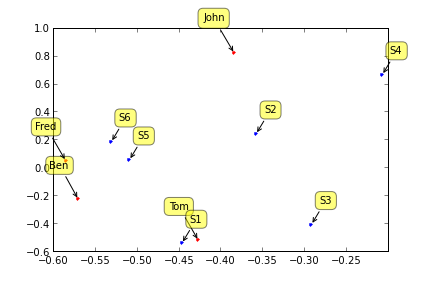
\includegraphics[height=6cm]{svdrecom_1.png}

Çok güzel! SVD bize ürün bazında sezon 5 ve 6'nin bir küme
oluşturduğunu, Ben ve Fred'in de kişi bazında ayrı bir küme olduğunu
gösterdi.

Azaltılmış boyutları nasıl kullanırız? Yeni bir kişiyi (mesela Bob)
ele alınca, bu kişinin verisini öncelikle aynen diğer verilerin
indirgendiği gibi azaltılmış boyuta "indirgememiz" gerekiyor. Çünkü
artık işlem yaptığımız boyut orası. Peki bu indirgemeyi nasıl yaparız?
SVD genel formülünü hatırlarsak,

$$ A = USV $$

Azaltılmış ortamda

$$ A = U_k S_k V_k $$

Diyelim ki gitmek istediğimiz nokta azaltılmış $U$, o zaman $U_k$'yi tek
başına bırakalım (dikkat, mesela $V$'nin tersini aldık, fakat bir matrisin
tersini almak için o matrisin kare matris olması gerekir, eğer kare
değilse, ters alma işlemi taklit ters alma işlemi -pseudoinverse- ile
gerçekleştirilir, daha fazla detay için [6])

$$ A V_k^{-1} = U_k S V_k V_k^{-1} $$

$U_k,V_k$ matrisleri birimdik (orthonormal), o zaman $V_k^{-1}V_k = I$
olacak, yani yokolacak

$$ A V_k^{-1} = U_k S  $$

Benzer şekilde

$$  A V_k^{-1} S^{-1} = U_k $$

Çok fazla ters alma işlemi var, her iki tarafın devriğini alalım

$$ (S^{-1})^T (V_k^{-1})^T A^T = U_k^T $$

$V_k^{-1} = V_k^T$ olduğunu biliyoruz. Nasıl? Çünkü $ V_k^TV_k = I $, aynı
şekilde $ V_k^{-1}V_k = I $. Ters alma işleminin özgünlüğü (üniqueness)
sebebiyle $V_k^{-1} = V_k^T$ olmak zorundadır $\Box$

Demek ki üstteki formül devriğin devriğini almak demektir, yani tekrar başa
dönmüş oluyoruz, demek ki $V_k$ değişmeden kalıyor

$$ (S^{-1})^T V_k A^T = U_k^T $$

$S$ ise köşegen matris, onun tersi yine köşegen, köşegen matrisin devriği
yine kendisi

$$ S^{-1} V_k A^T = U_k^T $$

Bazı kod ispatları, $u$'nun birimdik olması:

\begin{minted}[fontsize=\footnotesize]{python}
print np.dot(u.T,u)
\end{minted}

\begin{verbatim}
[[  1.00000000e+00   4.83147593e-18]
 [  4.83147593e-18   1.00000000e+00]]
\end{verbatim}

Doğal olarak \verb!1e-17! gibi bir sayı sıfıra çok yakın, yani sıfır kabul
edilebilir. Devrik ve tersin aynı olduğunu gösterelim: İki matrisi birbirinden
çıkartıp, çok küçük bir sayıdan büyüklüğe göre filtreleme yapalım, ve sonuç
içinde bir tane bile True olup olmadığını kontrol edelim,

\begin{minted}[fontsize=\footnotesize]{python}
print not any(U.T-la.inv(U) > 1e-15)
\end{minted}

\begin{verbatim}
True
\end{verbatim}

Yeni Bob verisi 

\begin{minted}[fontsize=\footnotesize]{python}
bob = np.array([5,5,0,0,0,5]) 
\end{minted}

O zaman 

\begin{minted}[fontsize=\footnotesize]{python}
print bob.T.shape
print u.shape
S_k = np.eye(2)*Sigma[:2]
bob_2d = np.dot(np.dot(la.inv(S_k),vt.T),bob.T)
print bob_2d
\end{minted}

\begin{verbatim}
(6,)
(4, 2)
[-0.37752201 -0.08020351]
\end{verbatim}

Not: \verb!bob.T! üstteki formüldeki $A^T$ yerine geçecek; formülü tekrar
düzenlerken $A$ üzerinden işlem yaptık, fakat formülü ``$A$'ya eklenen
herhangi bir yeni satır'' olarak ta görebiliriz, ki bu örneğimizde Bob'un
verisi olurdu. 

Üstte \verb!eye! ve \verb!Sigma! ile ufak bir takla attık, bunun sebebi
\verb!svd! çağrısından gelen \verb!Sigma!  sonucunun bir vektör olması ama
üstteki işlem için köşegen bir "matrise" ihtiyacımız olması. Eğer birim
(identity) matrisini alıp onu \verb!Sigma! ile çarparsak, bu köşegen
matrisi elde ederiz.

Şimdi mesela kosinüs benzerliği kullanarak bu izdüşümlenmiş yeni
vektörün hangi diğer vektörlere benzediğini bulalım.

\begin{minted}[fontsize=\footnotesize]{python}
for i,user in enumerate(u):
   print data.index[i],cos_sim(user,bob_2d)
\end{minted}

\begin{verbatim}
Ben 0.993397525045
Tom 0.891664622942
John 0.612561691287
Fred 0.977685793579
\end{verbatim}

Sonuca göre yeni kullanıcı Bob, en çok Ben ve Fred'e benziyor. Sonuca
eriştik! Artık bu iki kullanıcının yüksek not verdiği ama Bob'un hiç
not vermediği sezonları alıp Bob'a tavsiye olarak sunabiliriz.

SVD ile Veriyi Oluşturmak

\begin{minted}[fontsize=\footnotesize]{python}
import pandas as pd
import numpy.linalg as lin
import numpy as np
import scipy.sparse.linalg as lin
import scipy.sparse as sps

d =  np.array(
[[ 5.,  5.,  3.,  np.nan,  5., 5.],
 [ 5.,  np.nan,  4.,  np.nan,  4., 4.],
 [ np.nan,  3.,  np.nan,  5.,  4., 5.],
 [ 5.,  4.,  3.,  3.,  5., 5.],
 [ 5.,  5.,  np.nan,  np.nan,  np.nan, 5.]
])
users = ['Ben','Tom','John','Fred','Bob']
seasons = ['0','1','2','3','4','5']
data = pd.DataFrame (d, columns=seasons,index=users)
print data
avg_movies_data = data.mean(axis=0)
print avg_movies_data
data_user_offset = data.apply(lambda x: x-avg_movies_data, axis=1)
A = sps.coo_matrix(np.nan_to_num(np.array(data_user_offset)))
U,S,VT = lin.svds(A,k=3)
def predict(u,i):
    offset = np.dot(U[u,:],VT[:,i]) 
    r_ui_hat = offset + avg_movies_data.ix[i] 
    return r_ui_hat, offset

print 'Bob', predict(users.index('Bob'),2)
print 'Tom', predict(users.index('Tom'),1)
\end{minted}

\begin{verbatim}
       0   1   2   3   4  5
Ben    5   5   3 NaN   5  5
Tom    5 NaN   4 NaN   4  4
John NaN   3 NaN   5   4  5
Fred   5   4   3   3   5  5
Bob    5   5 NaN NaN NaN  5
0    5.000000
1    4.250000
2    3.333333
3    4.000000
4    4.500000
5    4.800000
dtype: float64
Bob (3.3115641365499888, -0.021769196783344661)
Tom (4.295419370813935, 0.045419370813934629)
\end{verbatim}

Alternatif Yöntem

Bir diğer yöntem [1] yeni Bob verisi $y$'yi alıp

$$ z = VV^Ty $$

olarak $z$'ye çevirmek. Bu durumda aslında cebirsel olarak hiçbir şey
yapmamış oluyoruz,

$$ z = VV^Ty = Iy = y$$

ve iteratif sayısal çoğu algoritmanın temelini de bu oluşturuyor. Kavramsal
olarak $y$'yi alıp $V$ uzayına ``yansıtıyoruz''. Daha kavramsal olarak kullanıcı
seçimlerini temsil eden veri için $V$ bir ``kordinat sistemi'' oluşturmuştur
(SVD'nin doğal sonucu olarak) ve her veri noktası bu kordinat sistemi, bu bazın
vektörlerinin bir kombinasyonu olarak temsil edilebilir durumdadır (SVD için
kullanılan veriden bahsediyoruz). Bu durumda yeni veriyi oraya yansıtmak doğal
bir işlemdir. Tabii yansıtıp sonra geri geliyoruz, yani başlangıçtaki boyutlara
/ hale dönüyoruz, bu olurken aynı zamanda Bob verisinin boş noktaları en makul
tahminlerle ``doldurulmuş'' oluyor.

\begin{minted}[fontsize=\footnotesize]{python}
from numpy.linalg import linalg as la
U,Sigma,V=la.svd(data, full_matrices=False)
print data.shape
print U.shape, Sigma.shape, V.shape
u = U[:,:2]
vt=V[:2,:].T
print data
print 'bob', bob
y = bob
for i in range(3):
    z = np.dot(vt,np.dot(vt.T,y))
    print z
    z[y>0] = y[y>0]
print z
\end{minted}

\begin{verbatim}
(4, 6)
(4, 4) (4,) (4, 6)
      S1  S2  S3  S4  S5  S6
Ben    5   5   3   0   5   5
Tom    5   0   4   0   4   4
John   0   3   0   5   4   5
Fred   5   4   3   3   5   5
bob [5 5 0 0 0 5]
[ 3.26615993  2.27206826  2.16256132  1.04609626  3.37952362  3.45858088]
[ 3.26615993  2.27206826  2.16256132  1.04609626  3.37952362  3.45858088]
[ 3.26615993  2.27206826  2.16256132  1.04609626  3.37952362  3.45858088]
[ 5.          5.          2.16256132  1.04609626  3.37952362  5.        ]
\end{verbatim}

Sonuca göre Bob büyük ihtimalle S5'i sevecektir, not tahminleri arasında en
yüksek puan orada tahmin edilmiş, ki bu daha önceki Ben ve Fred benzerlik
tahminleri ile uyumlu. 

Not: Döngüde $z$'nin hep aynı satır olması kafa karışıklığı yaratmasın, bu
çok ufak bir veri seti, daha büyük veri setlerdinde bu değişim
görülecektir. 

İteratif işlem sözde kod (pseudocode) olarak,

Algoritma \verb!imputed_svd!
\begin{enumerate}
  \item \verb!while! $z$'deki değişim azalıncaya kadar (convergence)
  \item $z = VV^Ty$ 
  \item  $y$'nin ilk halindeki bilinen noktaları alıp $z$'ye kopyala
\end{enumerate}

En son projemizde üstteki işlemin en iyi sonuçlar verdiğini gözlemledik. 

Movielens 1M Verisi

Bu veri seti 6000 kullanıcı tarafından yaklaşık 4000 tane filme
verilen not / derece (rating) verisini içeriyor, 1 milyon tane not
verilmiş, yani 4000 * 6000 = 24 milyon olasılık içinde sadece 1 milyon
veri noktası dolu. Bu oldukça seyrek bir matris demektir.

Verinin ham hali diğer ders notlarımızı içeren üst dizinlerde var, veriyi
SVD ile kullanılır hale getirmek için bu dizindeki \verb!movielens_prep.py!
adlı script kullanılır. İşlem bitince \verb!movielens.csv! adlı bir dosya
script'te görülen yere yazılacak. Bu dosyada olmayan derecelendirmeler,
verilmemiş notlar boş olacaktır. Bu boşlukları sıfırlarsak, seyrek matrisi
o noktaları atlar. Ardından bu seyrek matris üzerinde seyrek SVD
işletilebilir. Bu normal SVD'den daha hızlı işleyecektir.

Tavsiye kodlamamız için yazının başında anlatılan tekniği kullanacağız, film
verisi üzerinde boyut azaltılması yapılacak, benzer kullanıcı bulunacak, ve
herhangi bir yeni kullanıcı / film kombinasyonu için bu diğer benzer
kullanıcının o filme verdiği not baz alınacak.

Veriyi eğitim ve test olarak iki parçaya böleceğiz. SVD eğitim bölümü
üzerinde işletilecek.

Bu bağlamda, önemli bir diğer konu eksik veri noktalarının SVD
sonuçlarını nasıl etkileyeceği. Sonuçta eksik yerler \verb!nan!,
oradan sıfır yapılıp ardından seyrek matris kodlaması üzerinden
"atlanıyor" olabilir, fakat bu değerler atlanıyor (yani hızlı
işleniyor, depolanıyor) olsa bile, onların sıfır olmasının bir anlamı
yok mudur? Evet vardır. Not bakımından sıfır da bir not'tur, ve bu
sebeple sonuçları istenmeyen biçimde etkileyebilir.

O zaman mevcut veriyi öyle bir değiştirelim ki verilmemiş notlar, yani
sıfır değerleri sonucu fazla değiştirmesin.

Bunu yapmanın yollarından biri her film için bir ortalama not değeri
hesaplamak, ve bu ortalama değeri o filme verilen tüm not
değerlerinden çıkartmaktır. Bu işleme "sıfır çevresinde merkezlemek"
ismi de verilir, hakikaten mesela film j için ortalama 3 ise, 5 değeri
2, 3 değeri sıfır, 2 değeri -1 haline gelecektir. Bu bir ilerlemedir
çünkü ortalama 3 değeri zaten bizim için "önemsiz" bir değerdir,
tavsiye problemi bağlamında bizim en çok ilgilendiğimiz sevilen
filmler, ve sevilmeyen filmler. Bu değerler sırasıyla artı ve eksi
değerlere dönüşecekler, ve SVD bu farklılığı matematiksel olarak
kullanabilme yeteneğine sahip.

Altta Pandas \verb!mean! çağrısı ile bu işlemin yapıldığını görüyoruz, dikkat,
Pandas dataframe içinde \verb!nan! değerleri olacaktır, ve Pandas bu değerleri
atlaması gerektiğini bilir, yani bu değerler ortalamaya etki etmez. Ardından
merkezleme işlemi eğitim verisi üzerinde uygulanıyor.

\begin{minted}[fontsize=\footnotesize]{python}
import pandas as pd, os
import scipy.sparse as sps
df = pd.read_csv("%s/Downloads/movielens.csv" % os.environ['HOME'] ,sep=';')
print df.shape
df = df.ix[:,1:] # id kolonunu atla
df = df.ix[:,:3700] # sadece filmleri al
df_train = df.copy().ix[:5000,:]
df_test = df.copy().ix[5001:,:]
df_train[np.isnan(df_train)] = 0.0
movie_avg_rating = np.array(df_train.mean(axis=0))
df_train = df_train - movie_avg_rating
dfs_train = sps.coo_matrix(df_train)

df_train = np.array(df_train)
df_test = np.array(df_test)

print df_train.shape
print df_test.shape

__top_k__ = 10
import scipy.sparse.linalg as slin
import scipy.linalg as la
U,Sigma,V=slin.svds(dfs_train,k=__top_k__)
print U.shape, Sigma.shape, V.shape
Sigma = np.diag(Sigma)
\end{minted}

\begin{verbatim}
(6040, 3731)
(5001, 3700)
(1039, 3700)
(5001, 10) (10,) (10, 3700)
\end{verbatim}

Altta test verisi üzerinde satır satır ilerliyoruz, ve her satır (test
kullanıcısı) içinde film film ilerliyoruz. "Verilmiş bir not" arıyoruz
(çoğunlukla not verilmemiş oluyor çünkü), ve bulduğumuz zaman artık
elimizde test edebileceğimiz bir şey var, o notu "sıfırlayıp" vektörün
geri kalanını azaltılmış boyuta yansıtıyoruz, ve sonra o boyuttaki tüm
diğer $U$ vektörleri içinde arama yapıyoruz, en yakın diğer
kullanıcıyı buluyoruz ve onun bu filme verdiği notu tahminimiz olarak
kullanıyoruz.

Altta eğer bulunan diğer kullanıcı o filme not vermemişse, basitleştirme
amaçlı olarak, o filmi atladık. Gerçek dünya şartlarında filme not vermiş
ve yakın olan (en yakın olmasa da) ikinci, üçüncü kullanıcılar bulunup
onların notu kullanılabilir. Hatta en yakın k tane kullanıcının ortalaması
alınabilir (o kullanıcılar kNN gibi bir metotla bulunur belki), vs.

\begin{minted}[fontsize=\footnotesize]{python}
def euclid(inA,inB):
    return 1.0/(1.0 + la.norm(inA - inB))
    
rmse = 0; n = 0
for i,test_row in enumerate(df_test):
    for j, test_val in enumerate(test_row):
        # nan olmayan bir not buluncaya kadar ara
        if np.isnan(test_val): continue	
        # bulduk, test satirini tamamen kopyala ve bulunan notu silerek
        # onu nan / sifir haline getir cunku yansitma (projection) oncesi
        # o notu 'bilmiyormus gibi' yapmamiz lazim. 
	curr = test_row.copy()
        curr[j] = np.nan
        curr[np.isnan(curr)] = 0.

	proj_row = np.dot(np.dot(la.inv(Sigma),V),curr)

	sims = np.array(map(lambda x: euclid(x, proj_row), U[:,:__top_k__]))
	isim = np.argmax(sims)

	# eger bulunan kullanici o filme not vermemisse atla
	if np.isnan(df.ix[isim, j]): continue

	# egitim verisinde notlar sifir etrafinda ortalanmis, tekrar
	# normal haline dondur
	est = df_train[isim, j]+movie_avg_rating[j]

	# gercek not
	real = df_test[i, j]

	print i, 'icin en yakin', isim, 'urun',j, 'icin oy', est, 'gercek', real
        rmse += (real-est)**2
        n += 1
	break # her kullanici icin tek film test et
    if i == 20: break # 20 kullanici test et

print "rmse", np.sqrt(rmse / n)
\end{minted}

\begin{verbatim}
0 icin en yakin 1903 urun 144 icin oy 5.0 gercek 5.0
1 icin en yakin 239 urun 144 icin oy 5.0 gercek 5.0
2 icin en yakin 2045 urun 844 icin oy 4.0 gercek 4.0
3 icin en yakin 4636 urun 0 icin oy 3.0 gercek 4.0
4 icin en yakin 139 urun 845 icin oy 4.0 gercek 5.0
5 icin en yakin 427 urun 1107 icin oy 4.0 gercek 5.0
6 icin en yakin 3620 urun 31 icin oy 4.0 gercek 4.0
7 icin en yakin 1870 urun 0 icin oy 4.0 gercek 3.0
8 icin en yakin 4816 urun 106 icin oy 5.0 gercek 5.0
9 icin en yakin 3511 urun 0 icin oy 3.0 gercek 4.0
10 icin en yakin 3973 urun 1212 icin oy 5.0 gercek 4.0
11 icin en yakin 2554 urun 287 icin oy 4.0 gercek 5.0
12 icin en yakin 4733 urun 31 icin oy 4.0 gercek 3.0
13 icin en yakin 2339 urun 9 icin oy 4.0 gercek 3.0
14 icin en yakin 3036 urun 10 icin oy 4.0 gercek 3.0
15 icin en yakin 2748 urun 253 icin oy 5.0 gercek 5.0
16 icin en yakin 450 urun 16 icin oy 4.0 gercek 4.0
17 icin en yakin 1133 urun 9 icin oy 5.0 gercek 2.0
18 icin en yakin 3037 urun 253 icin oy 5.0 gercek 4.0
19 icin en yakin 1266 urun 107 icin oy 3.0 gercek 3.0
20 icin en yakin 537 urun 253 icin oy 5.0 gercek 5.0
rmse 0.975900072949
\end{verbatim}

Sonuç fena değil. Tavsiye programlarında RMSE 0.9 civarı iyi olarak
bilinir, Netflix yarışmasında [3] mesela kazanan algoritma RMSE 0.85'e
erişmiştir.

Kaynaklar

[1] Grigorik, {\em SVD Recommendation System in Ruby},
    \url{http://www.igvita.com/2007/01/15/svd-recommendation-system-in-ruby}

[2] Harrington, P., {\em Machine Learning in Action}

[3] Wikipedia, {\em Netflix Prize},
    \url{http://en.wikipedia.org/wiki/Netflix_Prize}

[4] Stack Exchange, {\em How do I use the SVD in collaborative filtering?}, \url{http://stats.stackexchange.com/questions/31096/how-do-i-use-the-svd-in-collaborative-filtering}

[5] Anand, {\em MORE ON LINEAR STRUCTURE IN DATA, AND SINGULAR VALUE DECOMPOSITION},
    \url{https://anandoka.wordpress.com/tag/imputed-svd}

[6] Bayramlı, Lineer Cebir, {\em Ders 33}

[8] Bayramlı, Netflix / Movielens Film Verisi,
    \url{https://burakbayramli.github.io/dersblog/sk/2015/04/pandas-movielens-netflix-ratings.html}


    
\end{document}

